\section{DESARROLLO} 
Parte 1: Consultando Datos
\begin{itemize}
\subsection{ANALISIS}
\subsection{DISEÑO}
\subsection{PRUEBAS}
	\item Crear un proyecto de pruebas a nuestra solución.
	\item Dentro de la clase, agregamos el siguiente metodo ObtenerAlEstudianteConIDUno.
	\begin{figure}[htb]
\begin{center}
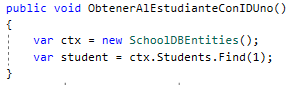
\includegraphics[width=12cm]{./Imagenes/1-1}
\end{center}
\end{figure}
	\item Agregamos el siguiente metodo BuscarAlPrimerEstudianteConElNombreBill.
\begin{figure}[htb]
\begin{center}
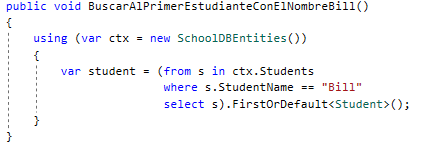
\includegraphics[width=12cm]{./Imagenes/1-2}
\end{center}
\end{figure}
	\item Agregamos el siguiente metodo BuscarEstudiantesAgrupadosPorEstandar.
\begin{figure}[htb]
\begin{center}
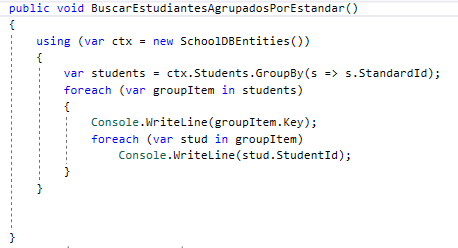
\includegraphics[width=12cm]{./Imagenes/1-3}
\end{center}
\end{figure}
	\item Agregamos el siguiente metodo ObetenerListadoDeEstudiantesOrdenadosPorNombre.
\begin{figure}[htb]
\begin{center}
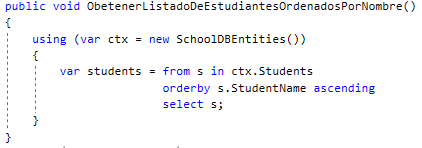
\includegraphics[width=12cm]{./Imagenes/1-4}
\end{center}
\end{figure}
	\item Agregamos el siguiente metodo BuscarTodosLostudiantesConElEstandarUno.
\begin{figure}[htb]
\begin{center}
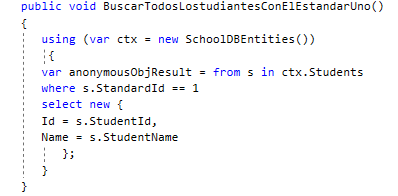
\includegraphics[width=12cm]{./Imagenes/1-5}
\end{center}
\end{figure}
\end{itemize}
Parte 2: Guardando Datos
\begin{itemize}
	\item Agregar al proyecto de pruebas una clase de pruebas TestUnit02, agregar el método
InsertarEstudianteSatisfactoriamente, tomar como referencia el siguiente código.
	\begin{figure}[htb]
\begin{center}
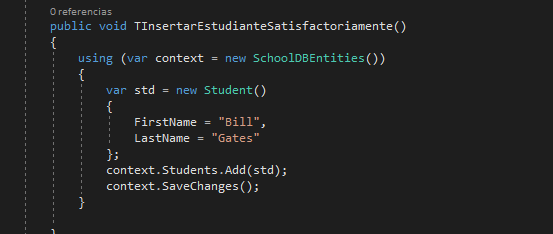
\includegraphics[width=12cm]{./Imagenes/1-6}
\end{center}
\end{figure}
	\item Agregar el método ActualizarElPrimerEstudianteSatisfactoriamente, tomar como referencia el siguiente
código.
\begin{figure}[htb]
\begin{center}
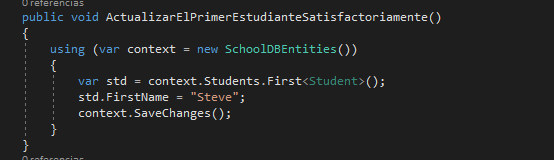
\includegraphics[width=12cm]{./Imagenes/1-7}
\end{center}
\end{figure}
	\item Agregar el método EliminarElPrimerEstudianteSatisfactoriamente, tomar como referencia el siguiente código.
\begin{figure}[htb]
\begin{center}
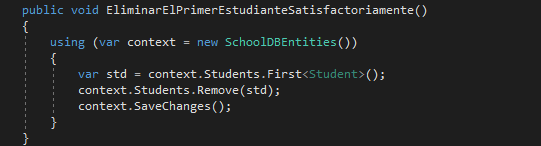
\includegraphics[width=12cm]{./Imagenes/1-8}
\end{center}
\end{figure}
	\item Agregar el método: AgregarTresEstudiantesSatisfactoriamente, tomar como referencia el siguiente código:

\begin{figure}[htb]
\begin{center}
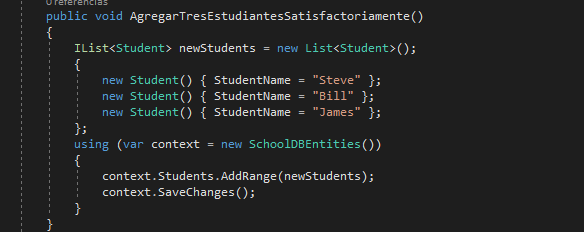
\includegraphics[width=12cm]{./Imagenes/1-9}
\end{center}
\end{figure}
	\item Finalmente agregar el método de pruebas: EliminarTresEstudiantesSatisfactoriamente, tomar como referencia el siguiente código:
\begin{figure}[htb]
\begin{center}
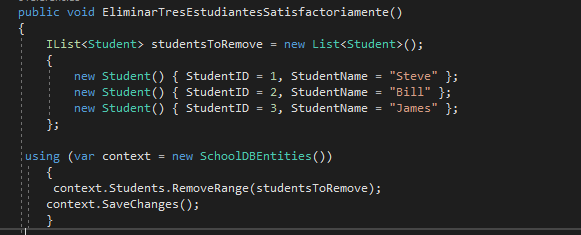
\includegraphics[width=12cm]{./Imagenes/1-10}
\end{center}
\end{figure}
\end{itemize}





